\documentclass[12pt, oneside]{extbook}
\usepackage[utf8]{inputenc}
\usepackage[russianb]{babel}
\newtheorem{theorem}{\protect\thmname}
\newcommand{\thmname}{}\newcommand{\exaname}{} % initialization
\addto\captionsrussian{
  \renewcommand{\thmname}{Теорема}
}
\usepackage{vmargin}
\setpapersize{A4}
\setmarginsrb{30mm}{20mm}{15mm}{20mm}{0pt}{0mm}{0pt}{13mm}
\usepackage{indentfirst}
\usepackage{setspace}
\setstretch{1.5}
\sloppy
\usepackage{graphicx}
\usepackage{amsfonts}
\graphicspath{ {./pics/} }
\usepackage{subfig}

\begin{document}
\pagenumbering{gobble}
\begin{figure}[h]

\includegraphics{MB}
\centering
\end{figure}
\center{
Московский государственный университет имени М.В. Ломоносова\\
Факультет вычислительной математики и кибернетики\\
Кафедра нелинейных динамических систем и процессов управления\\
}
\vspace*{3\baselineskip}
\center{
{\large Сивков Антон Александрович}\\
\medskip
{\Large \textbf{Применение нейроных сетей для моделирования объектов управления}}\\
\vspace*{3\baselineskip}
ВЫПУСКНАЯ КВАЛИФИКАЦИОННАЯ РАБОТА\\
}
\vspace*{4\baselineskip}
{\flushright
\textbf{
Научный руководитель:
}\\
д.ф-м.н., профессор\\
В. В. Фомичев\\
}
\vfill
\center{Москва, \the\year}
\clearpage
\pagenumbering{arabic}
\pagestyle{plain}
\setcounter{page}{2}
\tableofcontents
\begin{flushleft} \setlength{\parindent}{1cm}
\chapter{Введение}
\section{Постановка задачи}
Данная работа ставит целью сравнительный анализ способности нейронных сетей с различными архитектурами аппроксимировать объекты управления для задач идентификации, основное сравнение происходит в контексте способности сетей экстраполировать поведение объектов управления
\section{Виды идентификации}
В теории управления одной из основных задач является задача идентификации систем, задача построения математической модели объекта управления, способной адекватно воспроизводить реальное поведение объекта управления.
\par
Задачи идентификации приблизительно можно разделить на 3 вида:\\
\begin{itemize}
\item Модель 'белого ящика', модель применяется, когда точно известен основополагающий принцип, лежащий в основе устройства системы. Модель может применятся например для систем, описывающих взаимодействия в рамках законов Ньютона. Зачастую такие системы имеют сложную структуру, и для построения точной модели требуются неадекватные затраты времени.
\item Модель 'серого ящика', модель применяется, когда известны или имеются достачно сильные предположения о характере соотношений между входом и выходом системы, но остается некоторое количество 'свободных' параметров системы, которые приближаются с использованием данных выходов и входов системы. Модель может применятся, например для приближения параметров уравнения Моно при моделировании микробных популяций.
\item Модель 'чёрного ящика', модель применяется, когда сложно сделать какие-либо априорные предположения о структуре системы, в этой модели используются только данные о входах и выходах системы, модель применяется к различным нелинейным системам. В этой работе используется эта модель, нейронные сети обучаются моделировать 'черный ящик'. 
\end{itemize}
\par
Сама идея применения неронных сетей для моделирования объектов управления не нова, примеры можно найти в публикации \cite{fc90}, датированной 1990 годом, где простейшие сети используются для моделирования простых дискретных линейных объектов управления.
\section{Перцептрон Розенблатта}
\par
Имеет смысл дать краткую историю создания неронных сетей, и объяснить почему нейронные сети адекватно применять в широком спектре задач. 
\par
Одной из первых искусственных сетей, способных к перцепции (восприятию) и формированию реакции на воспринятый стимул, явился PERCEPTRON Фрэнка Розенблатта, предложенный им в 1957 году. Персептрон рассматривался его автором не как конкретное техническое вычислительное устройство, а как модель работы мозга. Нужно заметить, что после нескольких десятилетий исследований современные работы по искусственным нейронным сетям редко преследуют такую цель.\\
\begin{figure}[h]
\centering
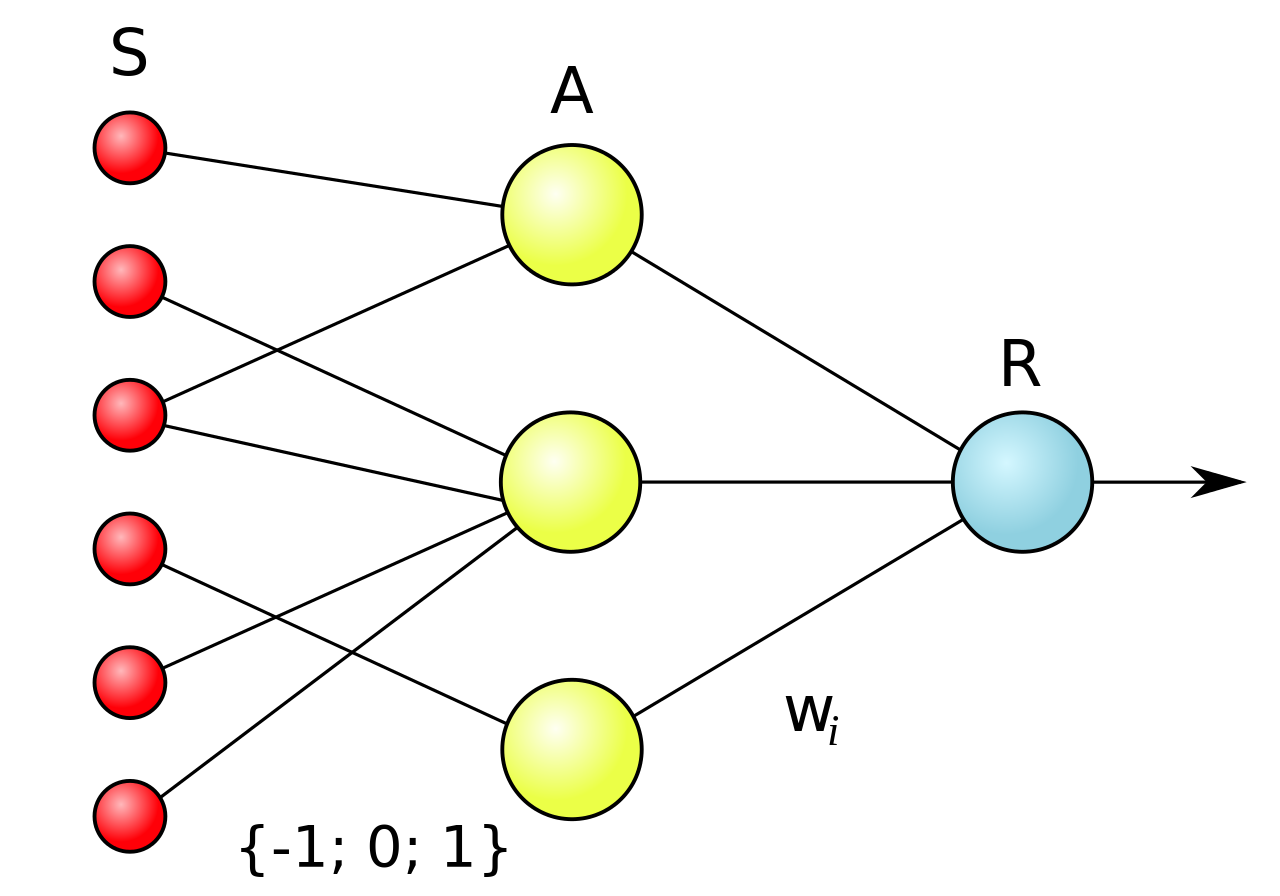
\includegraphics[width=0.4\textwidth]{perceptron}
\caption{Схема перцептрона.}
\label{fig:perceptron}
\end{figure}
\par
Стуктура перцептрона представлена на рисунке ~\ref{fig:perceptron}. Веса S--A связей могут иметь значения -1, +1 или 0 (то есть отсутствие связи), S-элементы воплощают собой слой сенсоров (рецепторов). В физическом воплощении они соответствуют, например, светочувствительным клеткам сетчатки глаза или фоторезисторам матрицы камеры. A-элементы называются ассоциативными, потому что каждому такому элементу, как правило, соответствует целый набор (ассоциация) S-элементов. A-элемент активизируется, как только количество сигналов от S-элементов на его входе превысило некоторую величину $\theta$. Сигналы от возбудившихся A-элементов, в свою очередь, передаются в сумматор R. Веса A--R связей W могут быть любыми. R-элемент, а вместе с ним и элементарный перцептрон, выдаёт «1», если линейная форма превышает порог $\theta$, иначе на выходе будет «-1». Перцептрон обучается правильно воспроизводить заданную функцию с помощью метода коррекции ошибок, в котором при ошибке веса изменяются на некоторую дельту, которая уменьшает ошибку на заданных данных. Розенблатт показал, что элементарный перцептрон, обучаемый по методу коррекции ошибки, независимо от начального состояния весовых коэффициентов и последовательности появления стимулов всегда приведёт к достижению решения за конечный промежуток времени.
\par
Важнейшим утверждением, которое частично объясняет и обосновывает сходимость большей части используемых сегодня нейронных сетей, является теорема об универсальной аппроксимации. Она формулируется так:\\
\begin{theorem}
\label{universal_approximation}
Пусть $\phi(\cdot)$ --- ограниченная, непостоянная монотонно возрастающая непрерывная функция. Пусть $I_{m_0}$ --- $m_0$--мерный единичный гиперкуб $[0, 1]^{m_0}$. Пусть пространство непрерывных на $I_{m_0}$ функций обозначается символом $C(I_{m_0})$.\\ Тогда $\forall f \in C(m_0)$ и $\varepsilon > 0$ $\exists\ m_1 \in \mathbb{Z}$~и~ множества~ $\{a_i\}, \{b_i\}, \{w_i\} \subset \mathbb{R}, i=1,...,m_1,\  j=1,...,m_0$, что:\\ $F\left(x_{1}, \ldots, x_{m_{0}}\right)=\sum_{i=1}^{m_{1}} a_{i} \phi\left(\sum_{j=1}^{m_{0}} w_{i j} x_{j}+b_{i}\right)$\\
является реализацией аппроксимации функции $f(\cdot)$, т.е.
$\left|F\left(x_{1}, \ldots, x_{m_{0}}\right)-f\left(x_{1}, \ldots, x_{m_{0}}\right)\right|<\varepsilon$
$\forall x_1,x_2,...,x_{m_0} \in I_{m_0}$\\
\end{theorem}
Теорема об универсальной аппроксимации непосредственно применима к многослойному персептрону. 
\par 
Хотя для простейших архитектур нейронных сетей сходимость доказуема, множество современных архитектур нейросетей не имеют под собой теоретической базы, котороя обосновывала бы их сходимость, тем не менее, они сходятся, и показывают впечатляющие результаты в задачах обработки речи, изображений, естественных языков, и многих других.\\
\section{Объект управления, использованный для экспериментов}
Для экспериментов использовался простейший объект управления, который можно описать следующей дискретной передаточной функцией:\\
\begin{equation} \label{eq:1}
H = \frac{z}{(z-\frac{1}{2})(z-\frac{1}{3})(z-\frac{1}{4})}
\end{equation}
\par
Объект устойчив, в экспериментах $dt = 1~sec$. Выглядит нелогичным проведение экспериментов, которые имеют смысл для сложных нелинейных объектов, на простейшем линейном дискретном объекте, однако данная работа имеет цель провести сравнительный анализ различных архитектур нейронных сетей, и, как показывает практика, даже такой простой объект позволяет сделать однозначные выводы относительно преимуществ одной архитектуры над другой.
\chapter{Моделирование с помощью многослойного перцептрона}
\section{Структура сети}
Многослойный перцептрон получил слово 'перцептрон' в названии в силу исторических причин, и его структура существенно отличается от структуры перцептрона Розенблатта, прежде всего тем, что он может иметь сколь угодно много слоев, и иметь обучаемые веса в каждом слое.
\begin{figure}[h]
\centering
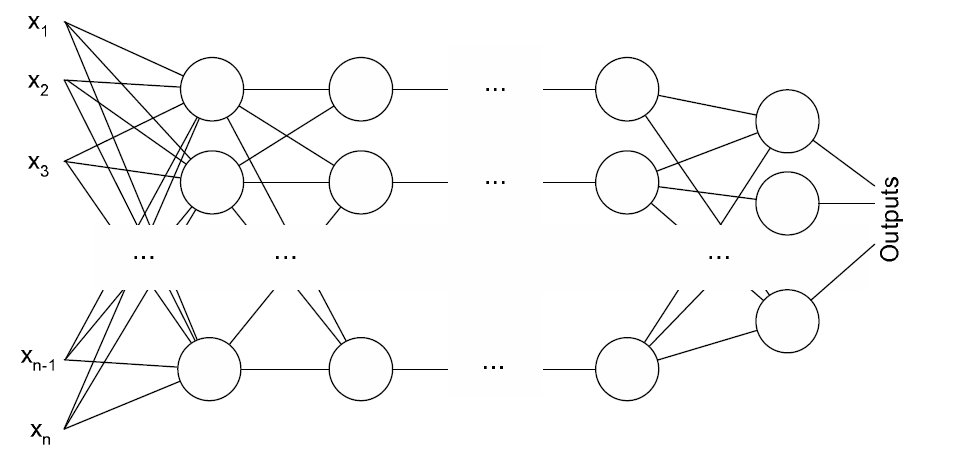
\includegraphics[width=0.5\textwidth]{multi_layer_perceptron_general}
\label{fig:multi_perceptron}
\caption{Многослойный перцептрон.}
\end{figure}
\par
Устройство перцептрона схематично представлено на рисунке \ref{fig:multi_perceptron}, $x_i$ обозначает i-й вход сети. Каждый из обозначенных на рисунке узлов сети выполняет следующее преобразование: $y = f(<w, x> + b)$, т. е. функция активации $f$ (как правило сигмоида, тангенс или ReLu), примененная к скалярному произведению вектора входов узла $x$ на вектор весов узла $w$ плюс сдвиг $b$ (bias). При обучении сети с помощью стохастического градиентного спуска веса изменяются на каждой итерации в направлении антиградиента функции ошибки предсказания сети $L(x, y, w)$ на текущих данных. Значение градиента вычисляется с помощью метода \textit{обратного распространения ошибки}. Этот метод вкратце можно описать так:\\
Пусть дан некий узел сети, для удобства отбросим функцию активации, т.к. она не влияет существенно на принцип вычислений. Пусть $y$ --- выход узла, $w_{i}$ --- веса узла, $x_{i}$ --- входы $i=1,...,n$, тогда справедливы следующие формулы:\\
\begin{equation} \label {eq:2}
\frac{\partial L}{\partial w_{i}} = \frac{\partial L}{\partial y} * \frac{\partial y}{\partial w_{i}} = \frac{\partial L}{\partial y} * x_{i}
\end{equation}\\
\begin{equation} \label {eq:3}
\frac{\partial L}{\partial x_{i}} = \frac{\partial L}{\partial y} * \frac{\partial y}{\partial x_{i}} = \frac{\partial L}{\partial y} * w_{i}
\end{equation}\\
Формула \ref{eq:1} позволяет вычислить производную ошибки по конкретному весу сети, если известна производная ошибки по выходу узла $\frac{\partial L}{\partial y}$, а формула \ref{eq:2} позволяет вычислить производную ошибки по выходам узлов, не являющихся выходными, путем рекурсивного рассчета производных по выходам, при этом рассчет происходит от выходов сети ко входам, в направлении, \textit{обратном} прямому вычислению.
\section{Код и схема модели}
\begin{figure}[h]
\centering
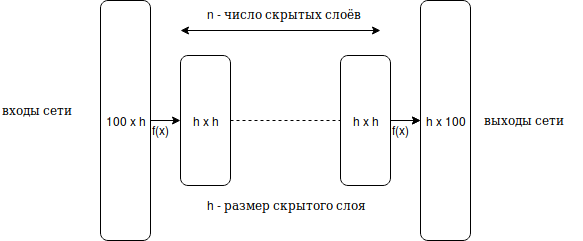
\includegraphics[width=0.8\textwidth]{multi_layer_perceptron}
\caption{Использованная для экспериментов архитектура}
\label{fig:my_multi_perceptron}
\end{figure}
Один из вариантов многослойного перцептрона, использованного для моделирования объекта управления \ref{eq:1} изображен на рисунке \ref{fig:my_multi_perceptron}, такой перцептрон может быть реализован на языке python с помощью библиотеки pytorch:
\pagebreak
\begin{verbatim}
class MultiPercNet(nn.Module):

    def __init__(self, input_size, output_size, n_layers, layer_size):
        super().__init__()
        self.layers = nn.ModuleList([nn.Linear(input_size, layer_size)])
        self.layers.extend(nn.Linear(layer_size, layer_size) for _ in range(n_layers - 2))
        self.layers.append(nn.Linear(layer_size, output_size))
        self.layer_size = layer_size
        for layer in self.layers:
            nn.init.xavier_uniform_(layer.weight, gain=1)
        self.input_size = input_size
        self.layer_size = layer_size
        self.tanh = nn.Hardtanh(min_val=-1, max_val=1)

    def forward(self, x):
        y = self.tanh(self.layers[0](x))
        for i in range(1, len(self.layers)):
            y = self.tanh(self.layers[i](y))
        return y
\end{verbatim}
\par
Сеть обучалась с использованием среднеквадратичной ошибки в качестве функции ошибки.
\pagebreak
\section{Эксперименты}
\begin{figure}[h]
\centering
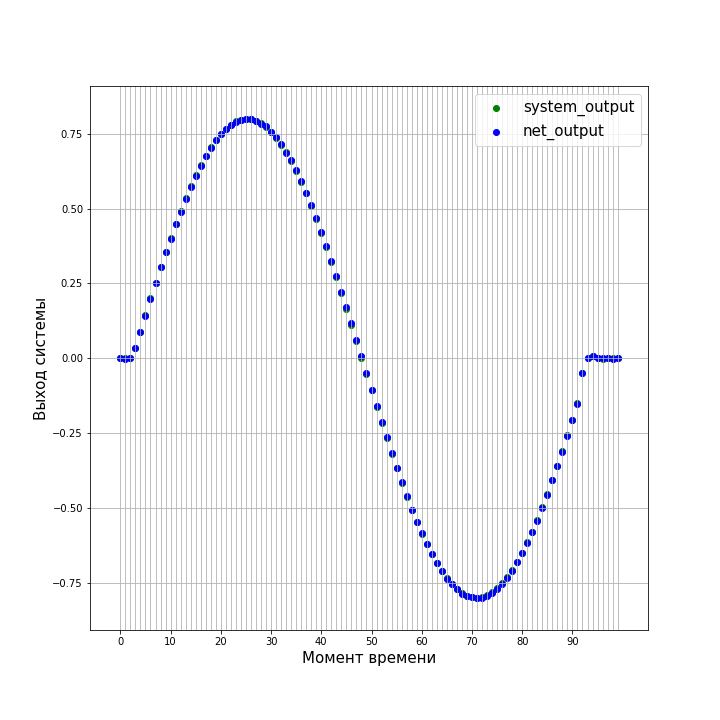
\includegraphics[width=0.9\textwidth]{fcnet_prediction}
\caption{Предсказание при отсутствии сдвига частот.}
\label{fig:multi_prediction}
\end{figure}
Во всех экспериментах сеть обучается на множестве входных и выходных сигналов системы, полученном при подаче на вход системы сигналов со случайной частотой, взятой из равномерного распределния на отрезке [0.05~Гц, 0.1~Гц], входные и выходные сигналы берутся за первые 100 секунд. На рисунке \ref{fig:multi_prediction} показано предсказание и реальный выход системы при подаче на вход системы сигнала со случайной частотой, полученной аналогично частоте входных сигналов, использованных при обучении. Среднеквадратичная ошибка при отсутсвии сдвига частот: 
$ 1.1196042208666767e-05$. Нетрудно заметить, что сеть предсказывает выход объекта управления практически идеально при сохранении той же частоты входных сигналов, что использовалась при обучении. Это объясняется тем, что объект управления имеет простейшую структуру, и сеть без проблем аппроксимирует выходной сигнал объекта управления при подаче входных сигналов, не выходящих за область данных, использованных для обучения.
\par
\begin{figure}[h]
\centering
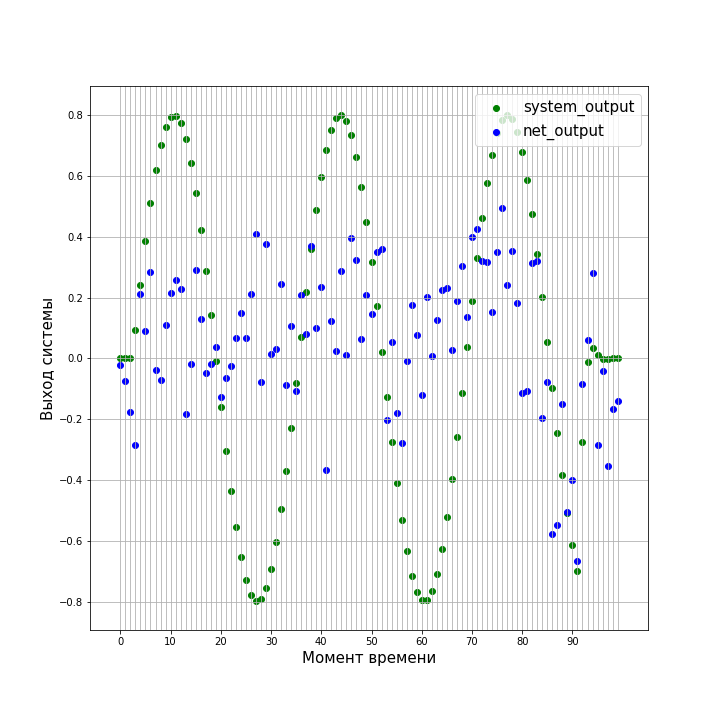
\includegraphics[width=0.9\textwidth]{fcnet_prediction_shifted}
\caption{Предсказание при частоте 0.2~Гц.}
\label{fig:multi_prediction_shifted}
\end{figure}
\
На рисунке \ref{fig:multi_prediction_shifted} изображено предсказание выхода системы сетью, обученной на входных и выходных данных, полученных при подаче на вход системы сигналов из того же диапазона частот [0.05~Гц, 0.1~Гц], при подаче на вход сигнала с частотой 0.2~Гц. Среднеквадратичная ошибка при подаче сигналов со случайной частотой из равномерного распределения [0.1~Гц, 0.2~Гц]: $ 0.19516661121453216$. Из показателей и рисунка \ref{fig:multi_prediction_shifted} можно сделать вывод о том что сеть не способна предсказать в какой--либо степени релевантные данных при выходе частоты входного сигнала за пределы параметров обучающей выборки. Это также позволяет сделать вывод о том, что сеть переобучается на данных обучающей выборки, и теряет способность к какой--либо экстраполяции поведения объекта управления. 
\par
\begin{figure}[!ht]
     \subfloat[Перебор размера скрытого слоя сети]{
         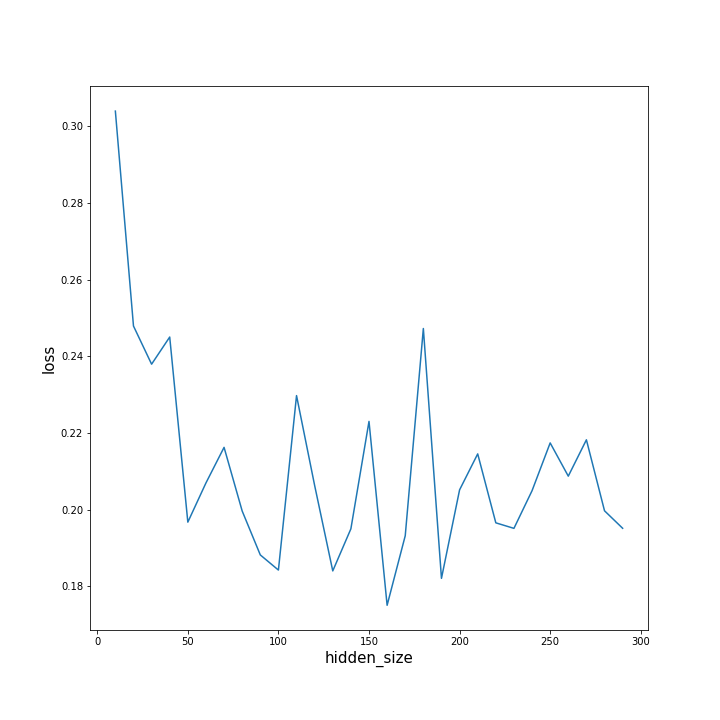
\includegraphics[width=0.45\textwidth]{perceptron_hiddden_size_search}
     }
     \hfill
     \subfloat[Перебор количества внутренних слоев]{
         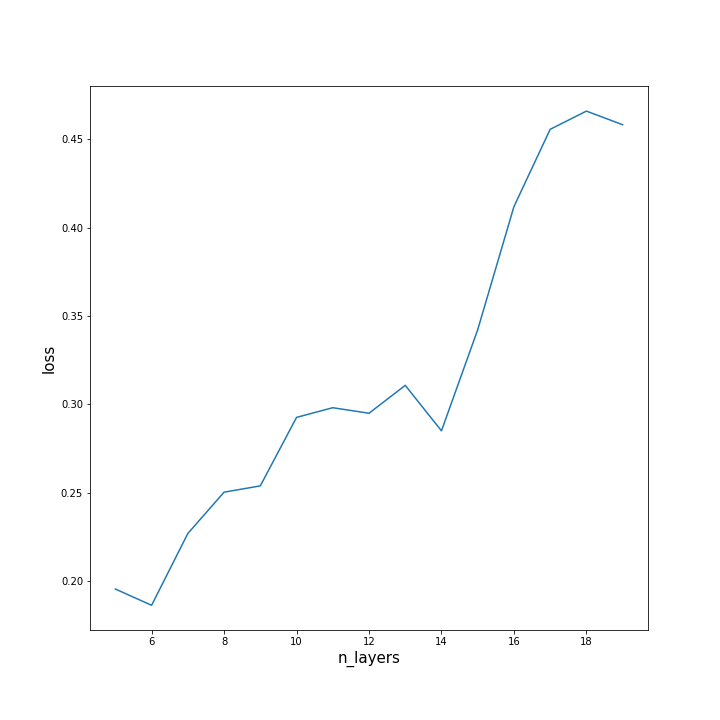
\includegraphics[width=0.45\textwidth]{perceptron_n_layers_search}
     }
     \centering
     \subfloat[Перебор функций активации]{
         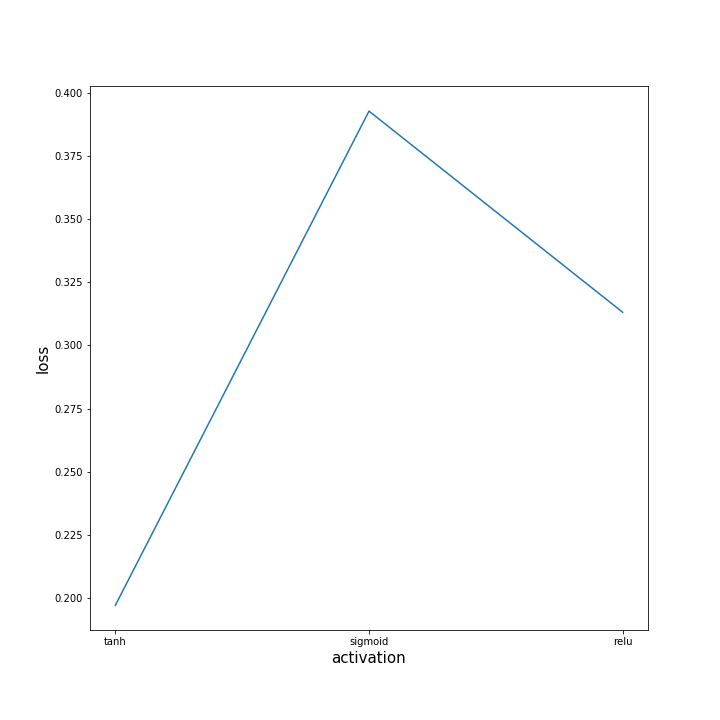
\includegraphics[width=0.45\textwidth]{perceptron_activation_search}
     }
     \caption{Перебор гиперпараметров}
     \label{fig:multi_perceptron_search}
\end{figure}
На рисунке \ref{fig:multi_perceptron_search} изображены графики значений 

\begin{thebibliography}{1}
\bibitem{fc90} KUMPATI S. NARENDRA FELLOW, IEEE. AND KANNAN  PARTHASARATHY, Identification and control of dynamical systems using neural networks, 1990, https://ieeexplore.ieee.org/abstract/document/80202
\end{thebibliography}
\end{flushleft}
\end{document}
